\documentclass{tufte-handout}
\usepackage{tikz}\usetikzlibrary{decorations.pathreplacing,positioning,chains}
\usepackage{tipa}
\usepackage{color}
\usepackage{listings}
\usepackage{amsmath}
\usepackage{booktabs}

\input{vc.tex}


\usepackage[lastexercise,answerdelayed]{exercise}
\setlength{\Exesep}{.5ex}
\setlength{\Exetopsep}{1em}
\renewcommand{\ExerciseListName}{Exercise}
\renewcommand{\AnswerListName}{}
\renewcommand{\ExerciseHeaderTitle}{(\emph{\ExerciseTitle.})\ }
\renewcommand{\ExerciseListHeader}{\ExerciseHeaderDifficulty%
\textbf{\ExerciseListName\ExerciseHeaderNB.}\ \ExerciseHeaderTitle%
\ExerciseHeaderOrigin\ignorespaces}
\renewcommand{\AnswerListHeader}{\textbf{\ExerciseHeaderNB.\ }}

\title{Amortised analysis}
\author{Thore Husfeldt}
\date{\small Revision {\tt \GITAbrHash}$\ldots$, \GITAuthorDate, \GITAuthorName}
\begin{document}
\maketitle
\begin{abstract}
  This note covers the technique of amortized analysis, as a
  supplement to [SW], the textbook \emph{Algorithms, 4th ed.} by
  Sedgewick and Wayne.

  It contains a complete answer to exercise 1.4.32 thus completing the
  proof of proposition~E in section 1.4.
\end{abstract}

\section{Resizing array}
\label{sec-1.1}

Consider the resizing array implementation of {\tt Stack} (Algorithm
1.1) and the collowing claim:

   
\begin{quote} {\bf Proposition A1.} In the resizing array
  implementation of {\tt Stack} (Algorithm 1.1), the average number of
  array accesses per operation for any sequence of {\tt push()} operations starting
  from an empty data structure is constant in the worst case.
\end{quote}

This is a true statement, and proved in [SW].

Is A1 still true when I remove ``starting from an empty data
structure''?
No.
To see this, begin with a stack that is the result of $2^k-1$
applications of {\tt push(null)}. 
Now {\tt N} equals $2^k-1$ and {\tt  a.length} equals $2^k$. 
From this starting position, a single {\tt push()} will will result in
a {\tt resize()}, leading to a  number of array accesses that is
linear in {\tt N}.
   
Is A1 still true when I remove ``average''?
No.
The same example works.
   
What we will do now is to show that A1 is still true when I remove
``{\tt push()}''. 
(This is exactly Proposition~E in [SW1].)
Intuitively, this sounds reasonable, since {\tt pop()} only makes the
stack smaller, whereas the expensive operation seems to happen when
the stack grows and causes and expensive {\tt resize()}.
However, even though this argument sounds tempting, it is wrong.
This is the purpose of the next example.
  
\subsection*{Stingy resizing array}
\label{sec-1.2}

We will change algorithm~1.1 to halve the size of {\tt a} as soon as
it can.  
More specifically, let algorithm~1.1' be the same as algorithm 1.1,
with the following change in the implementation of {\tt pop()}, where
a {\tt 4} was replaced by a {\tt 2}:

\begin{quote}
  {\tt if (N > 0 \&\& N == a.length/2) resize(a.length/2);}
\end{quote}
   
The implementation remains \emph{correct}, and it will also save
space. 
However, we can no longer guarantee the performance of proposition~E:

\begin{ExerciseList}\small
  \Exercise Exhibit a sequence of operations for which
  algorithm~1.1' requires a quadratic number of array accesses.
\end{ExerciseList}

In other words, the sequence requires a linear number of array
accesses on the average, much worse than the constant number
prophesised by proposition~E. 
We must resign ourselves to the fact that proposition~E does not hold
for algorithm~1.1'.
Since it does hold for algorithm~1.1 (I promise), the argument
somewhere must be sensitive to the difference between 4 and 2.
Our intuitive argument did not do this.

\subsection{Terminology: Amortisation and average}

From now on, we will try to avoid the term ``on the average.'' 
Not because it is wrong, but because it is too broad.
For more precision, we introduce the concept of ``amortised cost'',
borrowing terminology from the world of finance.\footnote{
{\bf amortize} 
/\textipa{"\ae m@r""taIz}, \textipa{@"mOrtaIz}/
verb [trans.]
reduce or extinguish an amount by money regularly put aside:
\emph{loan fees can be amortized over the life of the mortgage.}, gradually write off the initial cost of an asset: \emph{they want to amortize the tooling costs quickly}.
}
\footnote{Many people view this material as  difficult, subtle, and somewhat
boring. It may be well
characterised by a word whose latin root is \emph{ad mortis}, ``to death.''}

The idea is to ``write off'' the costs for {\tt reduce()} in the long
run by showing that, even though a particular call may be costly,
these expensive calls happen with such low frequency that by instead
charging a slight cost to every operation, the expensive operation
will be paid.

As with many good analogies, there is a pitfall: 
In banking it is perfectly acceptable to expend a large amount of
money immediately, and amortise it later, for example, buying a house
off a large loan, or amortising the expense of a good-quality tool
after many uses.
In contrast, this is not acceptable in the analysis of algorithms:
We will insist that every expensive operation is already paid (in
small rates) beforehand.\footnote{Another place where the banking
  analogy breaks down is that banks charge interest. Algorithms don't.}
Maybe ``piggy bank'' analysis would have been a better term, but the
word is what it is.

So, to be quite precise, here is the definition:

\begin{quote}
  Let $T(N)$ be the worst-case\footnote{Note that both the sequence of
    operations, and the input, are chosen by our worst enemy.}  running
    time for any sequence of $N$ operations. The amortized time for
    each operation is $T(n)/n$.
\end{quote}


So why don't we just call it average?

Because averages can be many things. We could average over all
sequences of operations (say, call {\tt push()} and {\tt pop()} with
equal probability), or over all inputs (this is called ``average case
complexity'', and a difficult and active reseach area). If the
algorithm uses randomness, we could average over those random outcomes
(this is called expected running time). Amortized time is a
particular, precise, worst-case average over the number of operations.

\begin{ExerciseList}\small
  \Exercise A multiride ticket in the Danish amusement part Tivoli
  costs 200 DKK and is valid for 10 rides. What is the worst case cost
  for a single ride? What is the amortised cost for a ride?  
  \Exercise
  Bob is a runner. 
  He has been running 6~km every day of the week, except on Sundays.
  What is the amortised number of kilometers he runs per day?
  \footnote{If you want to nitpick: Bob started running on 23 March
    2005.}
  Worst case (assuming lazy is bad)?
  \Exercise
  Ran is also a runner.
  He rolls a die every morning and runs as many kilometers.
  What is the average number of kilometers Ran runs per day?
  Worst case? 
  Amortised?
\end{ExerciseList}

\subsection*{Proof of Proposition E}

We rephrase the claim with our new terminology:

   
\begin{quote}{\bf Proposition E.} 
  In the resizing array implementation of {\tt Stack} (Algorithm 1.1),
  the amortised number of array accesses per operation for any
  sequence of operations starting from an empty data structure is
  constant in the worst case.
\end{quote}

We will pretend that every array access costs one coin.  
We associate a (ficticious) piggy bank with our data structure and
make every call of {\tt push()} and {\tt pop()} deposit a certain
number of coins in the bank.  
(Determining how many coins is the technically difficult part of the
argument.) 
The aim is to have the pig finance every call of {\tt resize()}.

Let my pull the right constants out of my hat: {\tt push()} shall
deposit 8 coins, {\tt pop()} shall deposit 4 coin.%
\footnote{If you want to be precise {\tt push()} costs 9 coins. %
  It uses 1 coin to pay for the array access in line 2, and puts the
  others in the pig. %
  Similarly, {\tt pop()} costs 6 coins. %
  It uses 2 coins to pay for the array acccesses in its first two
  lines and puts the remainder in the pig.}

The difficulty are the two internal calls to {\tt resize()}.  
A call to {\tt resize(max)} requires $\mathtt{max}+ 2N$ array
accesses.\footnote{See the last Q\&A in section~1.4 for our convention
  about the cost of {\tt new}.}  
We can simplify this expression by observing that $\mathtt{max}=2N$
whenever {\tt resize()} is called.
To see this, look at the condition to $\mathtt{if}$ in both calls to
\texttt{resize()}: from inside \texttt{push()}, we have $\mathtt{max}=
\mathtt{2*a.length} = 2N$, and from inside \texttt{pop()} we have
$\mathtt{max}= \mathtt{a.length/2}= 2 \mathtt{a.length/4} = 2N$.
Thus, both calls of {\tt resize()} require $4N$ coins.  
We need to show that the pig can handle that.

We need to consider the very first call of {\tt resize()} separately.
This is an easy case.  
The data structure is initialised with $\mathtt{a.length}=1$ and
$N=0$, and the first call of {\tt resize()} must come from {\tt
  push()} when $N=1$.  
We need $4N=4$ coins, and have just deposited $8$ coins, so the charge
is easily paid.

Another easy observation will turn out to be useful, so I will pull
that out of my hat as well:
 Immediately after every call of {\tt
  resize()}, there are exactly $N$ occupied and $N$ free cells in {\tt
  a}: from looking at {\tt resize()} we can see is that there are
$\mathtt{max}-N$ free cells, and we already observed above that
$\mathtt{max}=2N$.
\begin{marginfigure}
  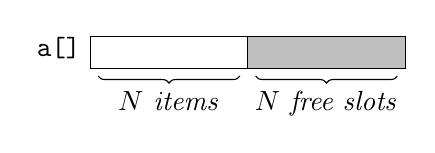
\begin{tikzpicture}
    \draw (0,0) 
          node[anchor=south east] {\texttt{a[]}}
          rectangle (2,.4);
    \draw [fill=gray!50] (2,0) rectangle (4,.4);
    \draw (1.9,-.1)[decorate, decoration=brace]
          -- node[below=2pt] {\textit{$N$ items}}
          (.1,-.1);
    \draw (3.9,-.1)[decorate, decoration=brace] 
          -- node[below=2pt] {\textit{$N$ free slots}} 
          (2.1,-.1);
  \end{tikzpicture}
  \caption{The data structure immediately after {\tt resize()}.}
\end{marginfigure}



With this observation, we can proceed to show that at the start of
every subsequent call of {\tt resize()}, there are at least $4N$ coins
in the bank.
\begin{itemize}
\item If the call came from \texttt{push()}, i.e., to prevent
  overflow, then there must have been at least $N/2$ calls to
  \texttt{push()} since the last \texttt{resize()}. Each
  \texttt{push()} deposited 8 coins, so there are $4N$ coins, as
  needed.
\begin{marginfigure}
  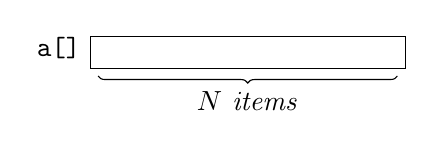
\begin{tikzpicture}
    \draw (0,0) 
          node[anchor=south east] {\texttt{a[]}}
          rectangle (4,.4);
    \draw (3.9,-.1)[decorate, decoration=brace]
          -- node[below=2pt] {\textit{$N$ items}}
          (.1,-.1);
  \end{tikzpicture}
  \caption{The data structure immediately before \texttt{push()} calls
    \texttt{resize()}.}
\end{marginfigure}
\item If the call came from \texttt{pop()}, i.e., to prevent underflow,
  then there must have been at least $N$ calls to \texttt{pop()} since
  the last \texttt{resize()}. Each \texttt{pop()} deposited 4 coins,
  so there are $4N$ coins, as needed.
\begin{marginfigure}
  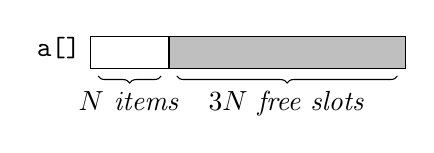
\begin{tikzpicture}
    \draw (0,0) 
          node[anchor=south east] {\texttt{a[]}}
          rectangle (1,.4);
    \draw [fill=gray!50] (1,0) rectangle (4,.4);
    \draw (0.9,-.1)[decorate, decoration=brace]
          -- node[below=2pt] {\textit{$N$ items}}
          (.1,-.1);
    \draw (3.9,-.1)[decorate, decoration=brace] 
          -- node[below=2pt] {\textit{$3N$ free slots}} 
          (1.1,-.1);
  \end{tikzpicture}
  \caption{The data structure immediately before \texttt{pop()} calls {\tt resize()}.}
\end{marginfigure}
\end{itemize}
This finishes the proof of proposition E.

\begin{ExerciseList}\small
  \Exercise \label{ex: only push}Can we charge all costs to
  \texttt{push()}? How much does it have to pay if \texttt{pop()} pays nothing?
  \Exercise Can we charge all costs to
  \texttt{pop()}? How much does it have to pay if \texttt{push()} pays nothing?
\end{ExerciseList}

\subsection{Localising the piggy bank argument}

Sometimes it is easier to localise the accounting argument by removing
the fictional piggy bank and depositing the coins in the data
structure instead.

For example, we can say that push operation puts 8 coins in the cell
it just filled, and every pop puts 4 coins in the cell that it just
freed. 

As before, when doubling the array from $N$ to $2N$, we argue that at
least $N$ {\tt push()} operations happened, so the entries in {\tt a}
from $N/2-1$ to $N$ contain at east 8 coins each, for a total of $4N$
coins. Similarly, for halving the array from $4N$ to $2N$, the calls
to {\tt pop()} put 4 coins on each of the free cells in $N+1,\ldots,
2N$, for a total of $4N$ coins. 

The local argument is sometimes attractive because there is a strong
inuition about what the coins will be doing, should they ever be
needed.  
For example, the 4 coins deposited by {\tt pop} in position {\tt
  a[N+1]} will be able to pay for the allocation of the new array
cells {\tt temp[1]} and {\tt temp[N+1]}, and the two accesses in {\tt
  temp[1] = a[1]}.

\begin{figure}
  \tikzstyle{cell}=[draw,on chain,minimum width=6mm,
  font=\tiny\tt, text height=1.25ex, text depth=.25ex]
  \tikzstyle{coin}=[draw,circle, on chain,inner sep= 1pt, fill=white,font=\tiny\sf]
  \begin{tikzpicture}[node distance=0cm]
    \begin{scope}[start chain]
      \node[on chain] {\tt a};
      \foreach \word in {to, be, or, not} \node [cell] {\word};
      \foreach \i in {4,...,7} \node [cell] {\it null};
    \end{scope}
    \node at (6,-.5) [anchor=west]{\tt pop(); pop();} ;
    \begin{scope}[start chain]
      \node at (0,-1) [on chain] {\tt a};
      \foreach \word in {to, be} \node (a\word) [cell]{\word};
      \foreach \i in {2,...,7} \node [cell](C\i) {\it null};
    \end{scope}
    \begin{scope}[start chain= going {at=(\tikzchainprevious),shift=(-80:.3)}]
      \node (N21) [coin,below of=C2] {N};
      \node (N22) [coin] {N};
      \node (R2) [coin] {R};
      \node (W2) [coin] {W};
    \end{scope}
    \begin{scope}[start chain= going {at=(\tikzchainprevious),shift=(-80:.3)}]
      \node (N31) [coin, below of=C3] {N};
      \node (N32) [coin] {N};
      \node (R3) [coin] {R};
      \node (W3) [coin] {W};
    \end{scope}
      \node at (6,-2) (TEMP) [anchor=west]{\tt temp = };
    \begin{scope}[start chain]
      \chainin (TEMP);
      \node [draw, red, on chain] (NEW) {\tt new Object[4];};
    \end{scope}
    \begin{scope}[start chain]
      \node at (0,-3) [on chain] {\tt temp};
      \foreach \i in {0,...,3} \node (NN\i) [cell] {\it null};
    \end{scope}
    \node at (6,-3.5) (TEMP0) [anchor=west,draw]{\tt temp[0] };
    \begin{scope}[start chain]
      \chainin (TEMP0);
      \node [on chain] {\tt = };
      \node [on chain, draw, red] (A0) {\tt a[0];};
  \end{scope}
  \node at (6,-4.3) (TEMP1) [anchor=west,draw]{\tt temp[1] };
  \begin{scope}[start chain]
    \chainin (TEMP1);
    \node [on chain] {\tt = };
    \node [on chain, draw, red] (A1) {\tt a[1];};
  \end{scope}    
  \begin{scope}[start chain]
      \node at (0,-5) [on chain] {\tt temp};
      \node (to) [cell] {to};   \node (be) [cell] {be};
      \foreach \i in {2,...,3} \node [cell] {\it null};
    \end{scope}
    \draw [->,nearly transparent] (N21) to[out=0,in=135] (NEW);
    \draw [->,nearly transparent] (N22) to[out=0,in=135] (NEW);
    \draw [->,nearly transparent] (N31) to[out=0,in=135] (NEW);
    \draw [->,nearly transparent] (N32) to[out=0,in=135] (NEW);
    \draw [->,nearly transparent] (R2) to (TEMP0);
    \draw [->,nearly transparent] (R3) to (TEMP1);
    \draw [->,nearly transparent] (W2) to (A0);
    \draw [->,nearly transparent] (W3) to (A1);
  \end{tikzpicture}
  % 
  \caption{ Two {\tt pop()} operations each deposit 4 coins (marked N, N, R,
    W), in {\tt a[2]} and {\tt a[3]} respectively.  When {\tt
      resize()} is called, the coins marked N are spent allocated the
    new array {\tt temp}, the R coin is spent reading from {\tt a},
    and the W coin is spent writing to {\tt temp}. In the new {\tt a}
    (which is {\tt temp}), there is no money.  }
\end{figure}

But it's a matter of taste. I like the local argument better for
exercise~\ref{ex: only push}.


\section{Mechanical Counter}

Whenever a mechanical counter is incremented, the rightmost wheel (the
``ones'') is turned. Every 10th increment, when the rightmost wheel
transitions from 9 to 0, its left neighbour is turned as well. This
effect continues to the left, so after $10^k-1$ increments, when the
counter shows $k$ 9s, the next increment will lead $k+1$ wheels to
turn.

\begin{figure}[htb]
\centerline{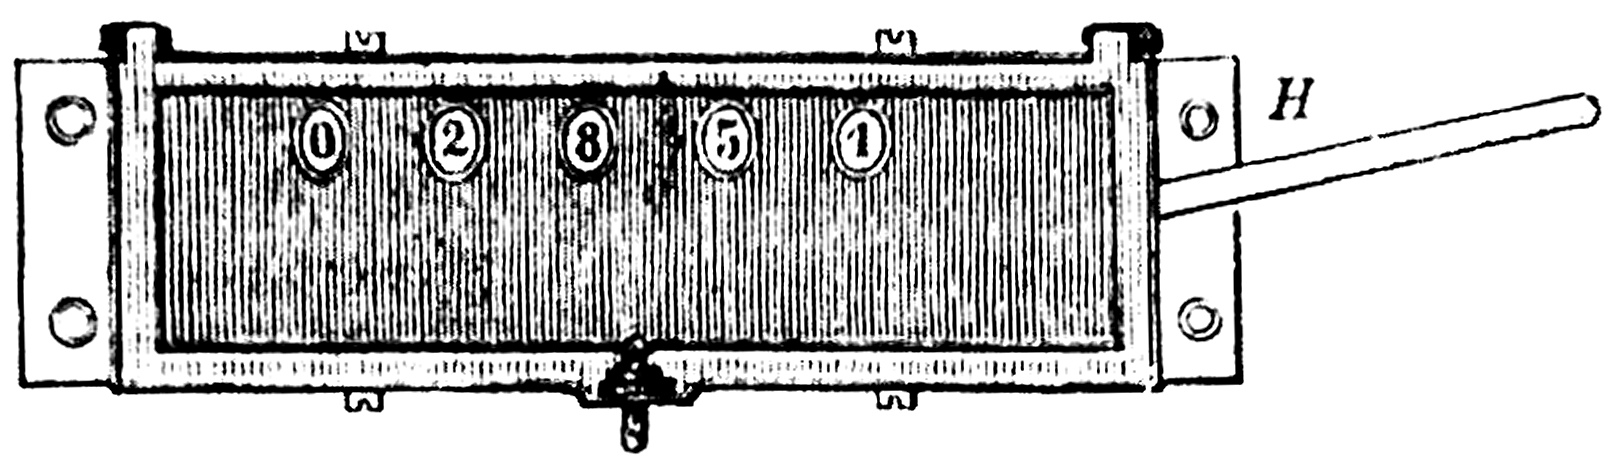
\includegraphics[width=2in]{Zaehlwerk_Schema_1.jpg}
$\quad$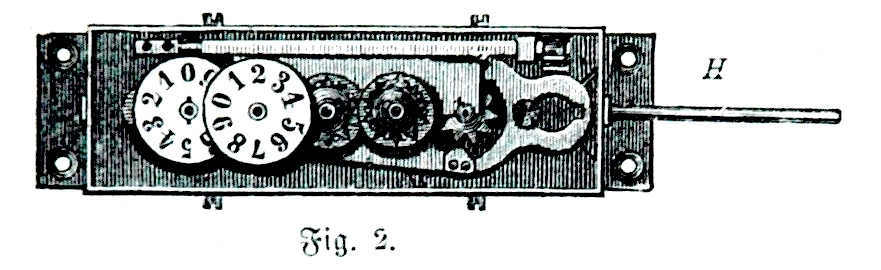
\includegraphics[width=2in]{Zaehlwerk_Schema_2_clean.png}}
\caption{A 5-digit mechanical counter.}
\end{figure}

In our terminology, the worst case number of operations for $N$
increments is logarithmic. But in the amortised sense, the behaviour
is much better:

\begin{quote}
  {\bf Proposition C.}  Starting from 0, a mechanical counter needs a
  constant amortised number of operations per increment.
\end{quote}

To establish this, we can use the ``easy'' aggregate method. Let
$N\geq 0$
be the total number of increments, and let us look at each wheel
separately. Number then $0,\ldots, k-1$ from right to left, so wheel~$0$
are the ones and $k=\lfloor \log_{10} N\rfloor$.

Wheel $0$ was rotated $N$ times. Wheel $1$ was rotated $\lfloor
N/10\rfloor$ times. In general, wheel $r$ was turned \[ \left \lfloor
\frac{N}{10^r} \right\rfloor\] times ($0\leq r < k$). Summing these
contributions for the total number of operations, gives 
\begin{multline*}
 \left \lfloor
\frac{N}{10^0} \right\rfloor +
 \left \lfloor
\frac{N}{10^1} \right\rfloor +
\cdots +
 \left \lfloor
\frac{N}{10^{k-1}} \right\rfloor
\leq \\
\frac{N}{10^0} +
\frac{N}{10^1} +
\cdots +
\frac{N}{10^{k-1}} 
=
N\left(\frac{1}{10^0}+\frac{1}{10^1}+\cdots+\frac{1}{10^{k-1}} \right)
< 2N.
\end{multline*}
This finishes the proof.

\begin{ExerciseList}\small
\Exercise
Prove proposition~C using the piggy bank method instead.
If you use the local argument, where does the money go?
How little do you actually need?
\footnote{To make this entertaining, assume it takes one pound
  sterling to turn a wheel and give the answer in pence.
  Next, assume it takes 1 shilling.}
\Exercise
 Assume the counter is built out of increasingly heavy material. 
 Each wheel costs twice as much to turn as the previous.
 (So, turning wheel 0 costs 1, wheel 1 costs 2, wheel 2 costs 4, 
 $\ldots$,  wheel $k$ costs $2^k$.)
 Does the analysis still work?
 What if wheel $k$ costs $10^k$? $11^k$?
\end{ExerciseList}

\section{Weighted quick-find}

\emph{This makes sense after [SW] 1.5}

\bigskip
We return to the first, very simple union-find data structure of [SW],
called \emph{quick-find}. 

Let us try to salvage this idea, at least partially. We're not going
to be able to beat the quick-union implementations, but this section
is mainly about \emph{analysis}, not so much about presenting the best
union--find algorithm known to Man.

Our first improvement is to make a clever choice about whether
\texttt{union(p, q)} renames {\tt p}'s component to {\tt q}'s or vice
versa. 
Our choice is to always rename the smaller component.
For this, we introduce another array {\tt int[] sz} to store component sizes, initially all $1$, and with the same meaning as in algorithm~1.4.

The second improvement is to link all elements of a component, so that we can quickly iterate over them when we want to rename them, instead of iterating over all of {\tt id}.
For this, we implement yet another array {\tt int[] next} of indices,
so that {\tt next[i]} is the element following {\tt i} in some
circular list of the component ids.

For example, the data structure looks like this after the operations
described by {\tt tinyUF.txt}.:

\medskip
{\tt \small
  \begin{tabular}{rcccccccccc}
      & 0 & 1 & 2 & 3 & 4 & 5 & 6 & 7 & 8 & 9 \\\midrule
id[] & 6 &6 &6 &4 &4 &6 &6 &6 &4 &4 \\
next[] & 5 &2 &0 &4 &9 &6 &7 &1 &3 &8 \\
sz[] &1 &1 &3 &1 &4 &1 &6 &1 &1 &1 
  \end{tabular}}
\medskip

Figure \ref{fig: WUF} shows the this situation, and the situation
after another call to {\tt union()}. 
An implementation is given in figure~\ref{fig: WUF impl}.

\begin{marginfigure}
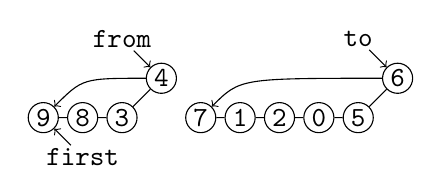
\begin{tikzpicture}[font=\tt,scale=.5,every node/.style={draw,circle,
    inner sep=1pt}]
  \node (9) at (0,0) {9};
  \node (8) at (1,0) {8};
  \node (3) at (2,0) {3};
  \node (4) at (3,1) {4};

  \node (7) at (4,0) {7};
  \node (1) at (5,0) {1};
  \node (2) at (6,0) {2};
  \node (0) at (7,0) {0};
  \node (5) at (8,0) {5};
  \node (6) at (9,1) {6};
  \draw[->] (7)--(1)--(2)--(0)--(5)--(6).. controls(5,1)..(7);
  \draw[->] (9)--(8)--(3)--(4)..controls(1,1)..(9);

  \node[draw=none,rectangle] at (1,-1) {first} edge [->] (9);
  \node[draw=none,rectangle] at (2,2) {from} edge [->] (4);
  \node[draw=none,rectangle] at (8,2) {to} edge [->] (6);
\end{tikzpicture}

\bigskip
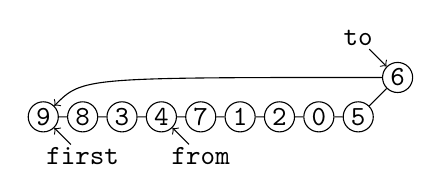
\begin{tikzpicture}[font=\tt,scale=.5,every node/.style={draw,circle,
    inner sep=1pt}]
  \node (9) at (0,0) {9};
  \node (8) at (1,0) {8};
  \node (3) at (2,0) {3};
  \node (4) at (3,0) {4};

  \node (7) at (4,0) {7};
  \node (1) at (5,0) {1};
  \node (2) at (6,0) {2};
  \node (0) at (7,0) {0};
  \node (5) at (8,0) {5};
  \node (6) at (9,1) {6};
  \draw[->]   (9)--(8)--(3)--(4)--(7)--(1)--(2)--(0)--(5)--(6)
  ..controls(1,1)..(9);

  \node[draw=none,rectangle] at (1,-1) {first} edge [->] (9);
  \node[draw=none,rectangle] at (4,-1) {from} edge [->] (4);
  \node[draw=none,rectangle] at (8,2) {to} edge [->] (6);
\end{tikzpicture}
\bigskip
\caption{\label{fig: WUF}{\tt union(1,8)}, where {\tt id[8] == 4} and {\tt id[1] ==
    6}.  The {\tt next} pointers are shown.}
\end{marginfigure}


\begin{figure}
\begin{tikzpicture}[remember picture,overlay] 
  \draw [fill=orange!30]
  (current page.south west) rectangle (current page.north east); 
\end{tikzpicture}

Algorithm A.1 Weighted quick-find implementation

\small
\begin{lstlisting}[basicstyle=\ttfamily,backgroundcolor=\color{white},
  frame=single,rulecolor=\color{gray!20},framesep=10pt, linewidth=12cm]
public class WeightedQuickFind
{
  private int[] id, sz, next;
  private int count;

  public WeightedQuickFind(int N)
  {
    count = N;
    id = new int[N];
    next = new int[N];
    sz = new int[N];
    for (int i = 0; i < N; i++) 
    { 
      id[i] = i;
      next[i] = i;
      sz[i] = 1;
    }
  }

  private void rename(int from, int to)
  {
    int first = next[from];
    for (int i = first; i != from; i = next[i])
	id[i] = to;
    id[from] = to;
    next[from] = next[to];
    next[to] = first;
    sz[to] += sz[from];
  }

  public void union(int p, int q) 
  {
    int pID = find(p); 
    int qID = find(q);
    if (pID == qID) return;
    if (sz[pID] < sz[qID]) rename(pID,qID);
    else                   rename(qID,pID);
    count--;
  }
  \\ see [SW], sect. 1.5 for find, count, connected, main
}
\end{lstlisting}
\caption{\label{fig: WUF impl}Weighted quick-find.}
\end{figure}


Intuitively, we have made our data structure a lot faster.
For instance, consider the sequence of $N$ unions in Figure~\ref{fig: fast sequence}.
\begin{marginfigure}
  \begin{tabbing}
    $N$\\
    {\tt 0 1}\\
    {\tt 1 2}\\
    {\tt 2 3}\\
    {\tt 3 4}\\
  $\vdots$\\
    $(N-2)$ $(N-1)$\\
  \end{tabbing}
\end{marginfigure}
Each {\tt union} takes constant time, whereas the original {\tt QuickFind} data structure would have used linear time.
This is great progress.
Unfortunately, our usual way of analyses is unable to detect that improvement, because we usually are interested in \emph{worst-case} running times.
And the worst case running time of {\tt WeightedQuickFind} is quite bad:

\begin{quote}
  {\bf Proposition.}
  A call to {\tt union()} in {\tt WeightedQuickFind} can take linear time in the worst case.
\end{quote}

\begin{marginfigure}
  \begin{tabbing}
    $N$\\
    {\tt 0 2}\\
    {\tt 1 3}\\
    {\tt 2 4}\\
    {\tt 3 5}\\
  $\vdots$\\
    $(N-4)$ $(N-2)$\\
    $(N-3)$ $(N-1)$\\
    $(N-2)$ $(N-1)$\\
  \end{tabbing}
\end{marginfigure}
To see that this is true, consider the sequence of operations in Figure~\ref{fig: slow}.
The very last call to union, when all the odd elements are united with the even elements, leads to $\tilde N$ array accessses.
(This happens in {\tt rename}, when the for-loop updates $\frac{1}{2}N$ entries in the {\tt id} array.)

Note that while this statement is true, it is also very pessimistic.

\begin{quotation}
  Before we continue, let's remind ourselves that there is a good reason for our usual focus on the worst case.
  We normally don't evaluate our data structure by its behaviour on particularly well-chosen inputs that make the data structure look good. 
  The \emph{best-case} time for {\tt QuickFind} was constant as well, after all: Just call {\tt union(0,1)} $N$ times in a row.

  Also note that `typical case' (however that should be defined) is a no-starter.
  Almost all calls to union in our two examples take constant time, so the `typical case behaviour is constant for {WeightedQuickFind}'---but that says more about our input sequences than the data structure.

  At this time one is tempted to define `average case,' or, to be quite precise `average input sequence.'
  This can indeed be done quite rigorously, by defining a random process.
  For instance, we could pick $p,q\in\{0,\ldots, N-1\}$ at random, independently and with the same probability, and then try to determine the expected value of the running time of {\tt union($p$,$q$)} after $N$ operations.
  There are two reasons for us to \emph{not} pursue this method of analysis.
  First, it is mathematically sophisticated and requires some exposure to discrete probability theory.
  Second, it tells us surprisingly \emph{little} about our data structure, because the result depends very heavily on the choice of distribution.
  (For instance, why should $p$ and $q$ be independent? 
  Why should they be uniformly distributed instead of normal, or Poisson, or a dozen other distributions that appear in real life?
  To appreciate these questions, imagine the union--find data structure used in an algorithm for Kruskal's algorithm for minimum spanning tree.
  Then the $p$ and $q$ depend on the structure of the input graph and the weight of its edges---that is absolutely not a uniformly random process!
  It would be much more interesting to define, say `the input sequence arising from the union--find calls of an execution of Kruskal's algorithm on a random graph.'
  But this gets \emph{very} difficult to analyse (including specific details about the implmentation!), and only shifts the question to `what kind or random process did the graph arise from'?
  No matter how we try to define `random inputs,' we find ourselves in the position of having to motivate the distribution.
  
  The discussion above largely served to motivate why we try to avoid the term `average.'
  It's not very well defined, and of very questionable value.
  (Moreover, we can't do the math.)
  )
\end{quotation}

\medskip
After rejecting all these methods of analysis we turn to amortised analysis.

\begin{quote}
  {\bf Proposition A4.} In the weighted quick-find implementation, {\tt union()} operation takes amortized logarithmic time in the worst case, beginning from an initialized data structure.
\end{quote}

We can show this using the aggregate method, so we consider a sequence of $k$ calls to {\tt union()} and want to show that it takes $O(k\log k)$ time.

We will count the number of updates of {\tt id[]} in {\tt rename()}, from the perspective of a single site $i$. 
The crucial observation is that whenever the {\tt id} of $i$ is renamed, the size of its component at least doubles.
(This is because we always rename the smaller of two unioned components, and the size of the union is at least twice of the smaller one.)
On the other hand, no component can ever be larger than $k+1$. 
(This is because every elemented started out in a component of its own.
At some time, that component must have been united with the others, which must have required a call to {\tt union()}.)
Thus, the component of $i$ has been doubled no more than $\log (k+1)$ times.
In particular, {\tt id[i]} has been changed at most $\log (k+1)$ times.

Next, we need to argue that at most $2k$ sites were renamed during the $k$ operations.
This is because a site that never appeared as one of the two arguments in some call to {\tt union} still remains in its original component.
Thus, at most $2k$ sites are ever renamed.
We argued above that just saw that each site gets renamed at most $\sim\log k$ times in total.
Thus, the total number of updates to {\tt id} is $\sim k\log k$. 
This finishes the proof of propostion A4.
\bigskip

Let us reiterate a few points about the formulation of proposition 4A:
\begin{enumerate}
  \item  Note the role that `worst case' plays:
    It says that in \emph{any}, even the most maliciously constructed input sequence, is is \emph{impossible} that the first $k$ operations take more than $O(k\log k)$ time in total.
    (Without `worst case', proposition A4 remains true, since it also holds for `best case' or `average case' or `typical case', however you want to define them.
    But none of those statements are interesting, and all of them are weaker.)
\item Note the role that `amortized' plays:
  Without it, proposition 4A is plainly false; there are operations that take linear time, as discussed above.
\item Note the role that `beginning from an initialized data structure' plays. 
  Without it, proposition 4A is plainly false; there are single operations that take linear time, as discussed above.
\end{enumerate}

\section{On the word `average' in [SW]}

We already discussed the use of the word `average' and its various meanings.
The concept described in these notes is a specific kind of average called `amortised,' and we have tried to be disciplined in our use of it.
This does not mean that the mental model of `amortisation is just some kind of average' is false.
In particular, the textbook [SW] itself uses the word in its own formulation of proposition A4.

However, as a possible source of confusion the word `average' is used in Proposition K in [SW, Sec. 2.3] with a different meaning:
\begin{quote}
  {\bf Proposition K}. Quicksort uses $\sim 2N\ln N$ compares (and one-sixth that many exchanges) on the average to sort an array of length $N$ with distinct keys.
\end{quote}
This statement describes the running time of a single run of an algorithm on a random input (namely, a sequence of uniformly and independently distributed integers).
This is precisely \emph{not} how `average' is used in proposition A4:
There, the sequence (which defines repeated operations on a data structure) is nonrandom (it is, in fact, a worst case sequence.)
\end{document}
